\section{Context Description}
The system described in this document, is a sluice type boat lift capable of fully autonomously transferring boats between two different levels (see Fig. \ref{fig:boat1}). In order to do so, the following steps have to be executed:\\ 

\noindent Assuming the system is in an idle state, which means both gates are closed, all signal lights indicate 'Halt', the water level inside the sluice is either equal to the top or bottom water level and the valve on that side is opened (to allow the water level inside to adapt to changes on the outside due to rain, tides etc.) while the other valve is closed. If a ship arrives at one of the signal lights, the sluice will detect it, check if the water level inside the sluice is at top or bottom and if necessary change it. Next, the gate on the ship's side will open and the entering signal light will switch to 'Pass', allowing the boat to enter. As soon as the boat is inside the sluice, this light will switch back to 'Halt', the gate will shut again and the boat will be transferred to the other level by closing one and opening the other valve. Once the target water level is reached, the gate on this side will open, the exit signal light will switch to pass and the ship can leave the sluice. If there is no other ship waiting to enter the sluice, the system will then return back to idle state.

\begin{figure}[!h]
	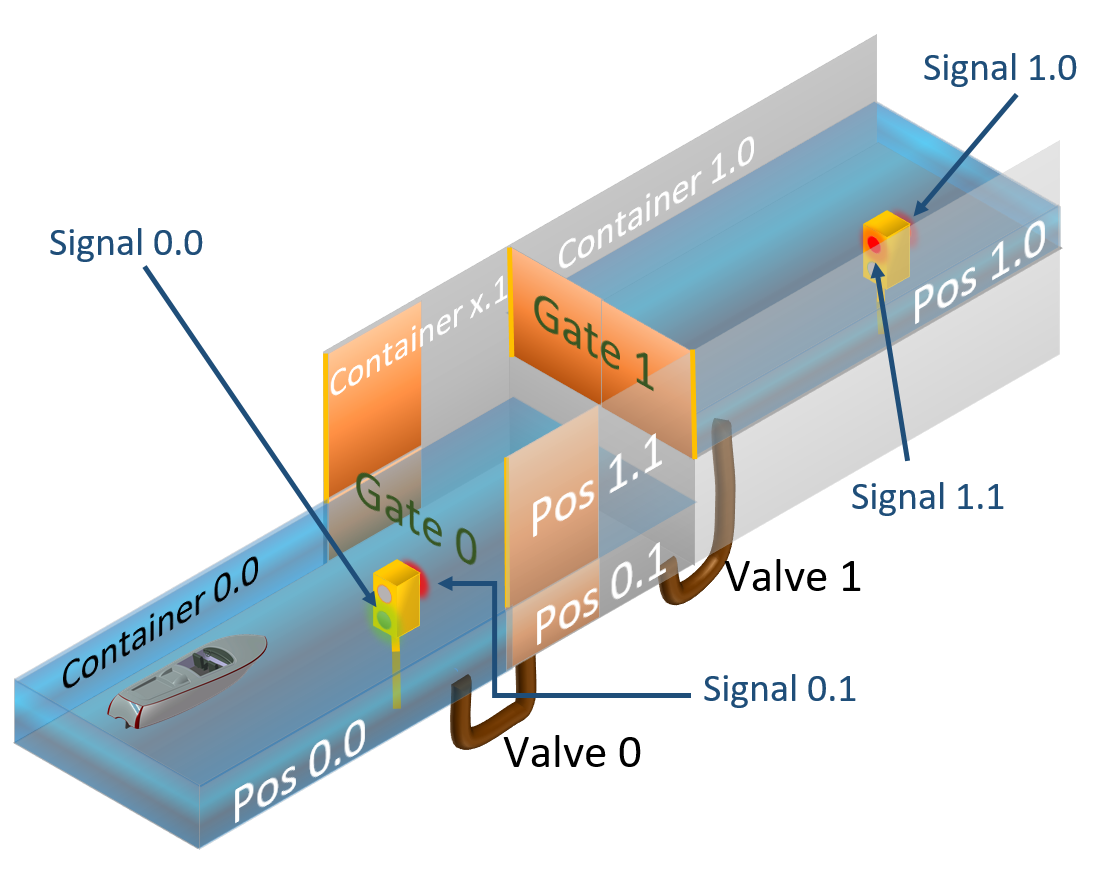
\includegraphics[width=\linewidth]{PictureName10}
	\caption{Detailed schematic of the system}
	\label{fig:boat1}
\end{figure}